\begin{abcliste}
\abc Die Beschleunigung ist die Steigung des $v(t)$-Graphen. Jedes Stück ist eine Gerade, $a$ ist darin konstant:
\begin{align}
 a_1 &= \aOneF = \frac{\vMax}{\tOne} = \aOne \approx \result{\aOneP{0}{1}} \\
 a_2 &= \result{0} \quad \text{(waagrecht)} \\
 a_3 &= \aThreeF = \frac{\vEnd-\vMax}{\tEnd-\tTwo} = \aThree \approx \result{\aThreeP{0}{1}}
\end{align}
Das $a(t)$-Diagramm besteht aus drei waagrechten Stücken mit Sprüngen bei \tOneO\ und \tTwoO:
\begin{center}
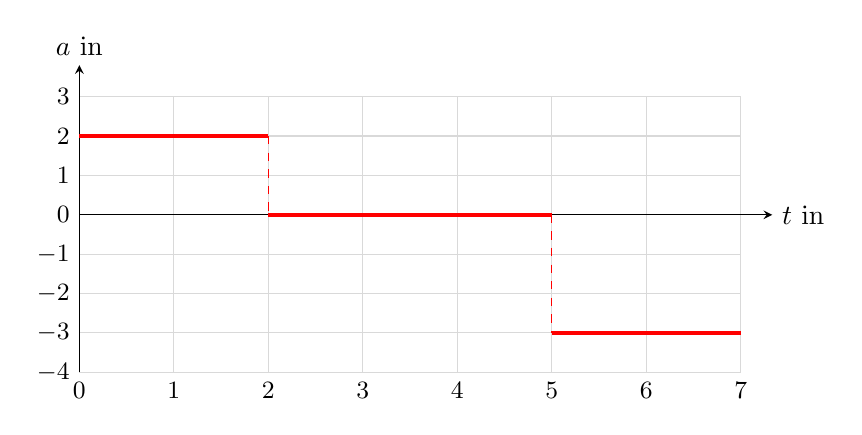
\begin{tikzpicture}[>=stealth, x=1.2cm, y=0.5cm]
 \draw[gray!30] (0,-4) grid[xstep=1, ystep=1] (7,3);
 \draw[->] (0,0) -- (7.333,0) node[right] {$t$ in \si{\second}};
 \draw[->] (0,-4) -- (0,3.8) node[above] {$a$ in \si{\meter\per\second\squared}};
 \foreach \tk in {0,1,2,3,4,5,6,7} \node[below] at (\tk,-4) {\small $\tk$};
 \foreach \yk in {-4,-3,-2,-1,0,1,2,3} \node[left] at (0,\yk) {\small $\yk$};

 \draw[ultra thick, red] (0,2) -- (2,2);
 \draw[ultra thick, red] (2,0) -- (5,0);
 \draw[ultra thick, red] (5,-3) -- (7,-3);
 \draw[red, dashed] (2,2) -- (2,0) (5,0) -- (5,-3);
\end{tikzpicture}
\end{center}
\abc Lea hat nicht recht. Die Geschwindigkeit wird bei
\begin{align}
 t &= \tZeroF = \tZero \approx \tZeroP{0}{2}
\end{align}
null, der Körper kehrt um und wird danach in die negative Richtung schneller. Die Steigung des $v(t)$-Graphen ist aber von \tTwoO\ bis \tEndO\ immer gleich: $\result{a = \aThreeP{0}{1}}$, vor und nach dem Umkehren. Ob der Körper schneller oder langsamer wird, hängt davon ab, ob $v$ und $a$ dasselbe Vorzeichen haben (schneller) oder verschiedene (langsamer), nicht vom Vorzeichen von $a$ allein.

Ben hat auch nicht recht: Er zeichnet die Werte von $v$ ab, statt die Steigung. Wo $v(t)$ steigt, ist $a$ konstant positiv; wo $v$ konstant ist, ist $a = 0$ (auch wenn $v$ dort gross ist); wo $v(t)$ fällt, ist $a$ konstant negativ.
\end{abcliste}
